\section{Sea Surface Velocity along Y-axis, (Vos, $v$) }
    \begin{frame}[plain]
        \vfill
      \centering
      \begin{beamercolorbox}[sep=8pt,center,shadow=true,rounded=true]{title}
        \usebeamerfont{title}\insertsectionhead\par%
        \color{oxfordblue}\noindent\rule{10cm}{1pt} \\
        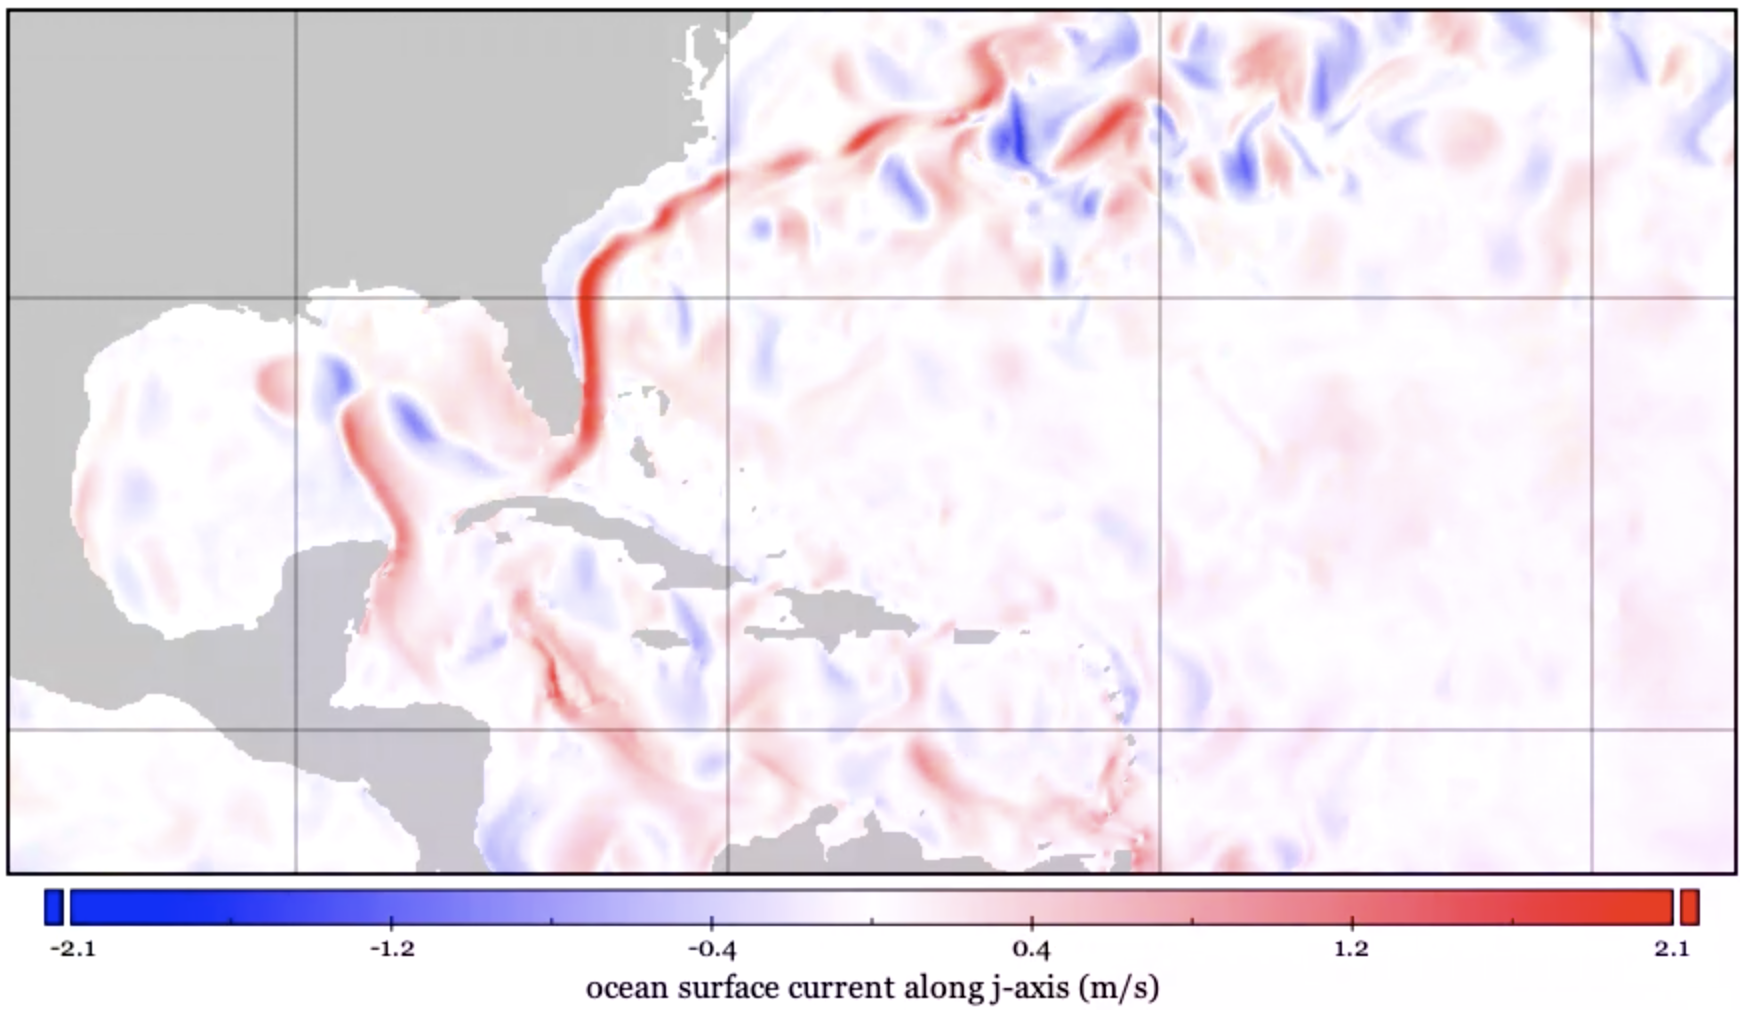
\includegraphics[width=0.93\linewidth]{images/example-images/vos.png}
      \end{beamercolorbox}
      \vfill
  \end{frame}

\section{Sea Surface Height above Reference Geoid (Zos, $\eta$, SSH) }
    \begin{frame}[plain]
        \vfill
      \centering
      \begin{beamercolorbox}[sep=8pt,center,shadow=true,rounded=true]{title}
        \usebeamerfont{title}\insertsectionhead\par%
        \color{oxfordblue}\noindent\rule{10cm}{1pt} \\
        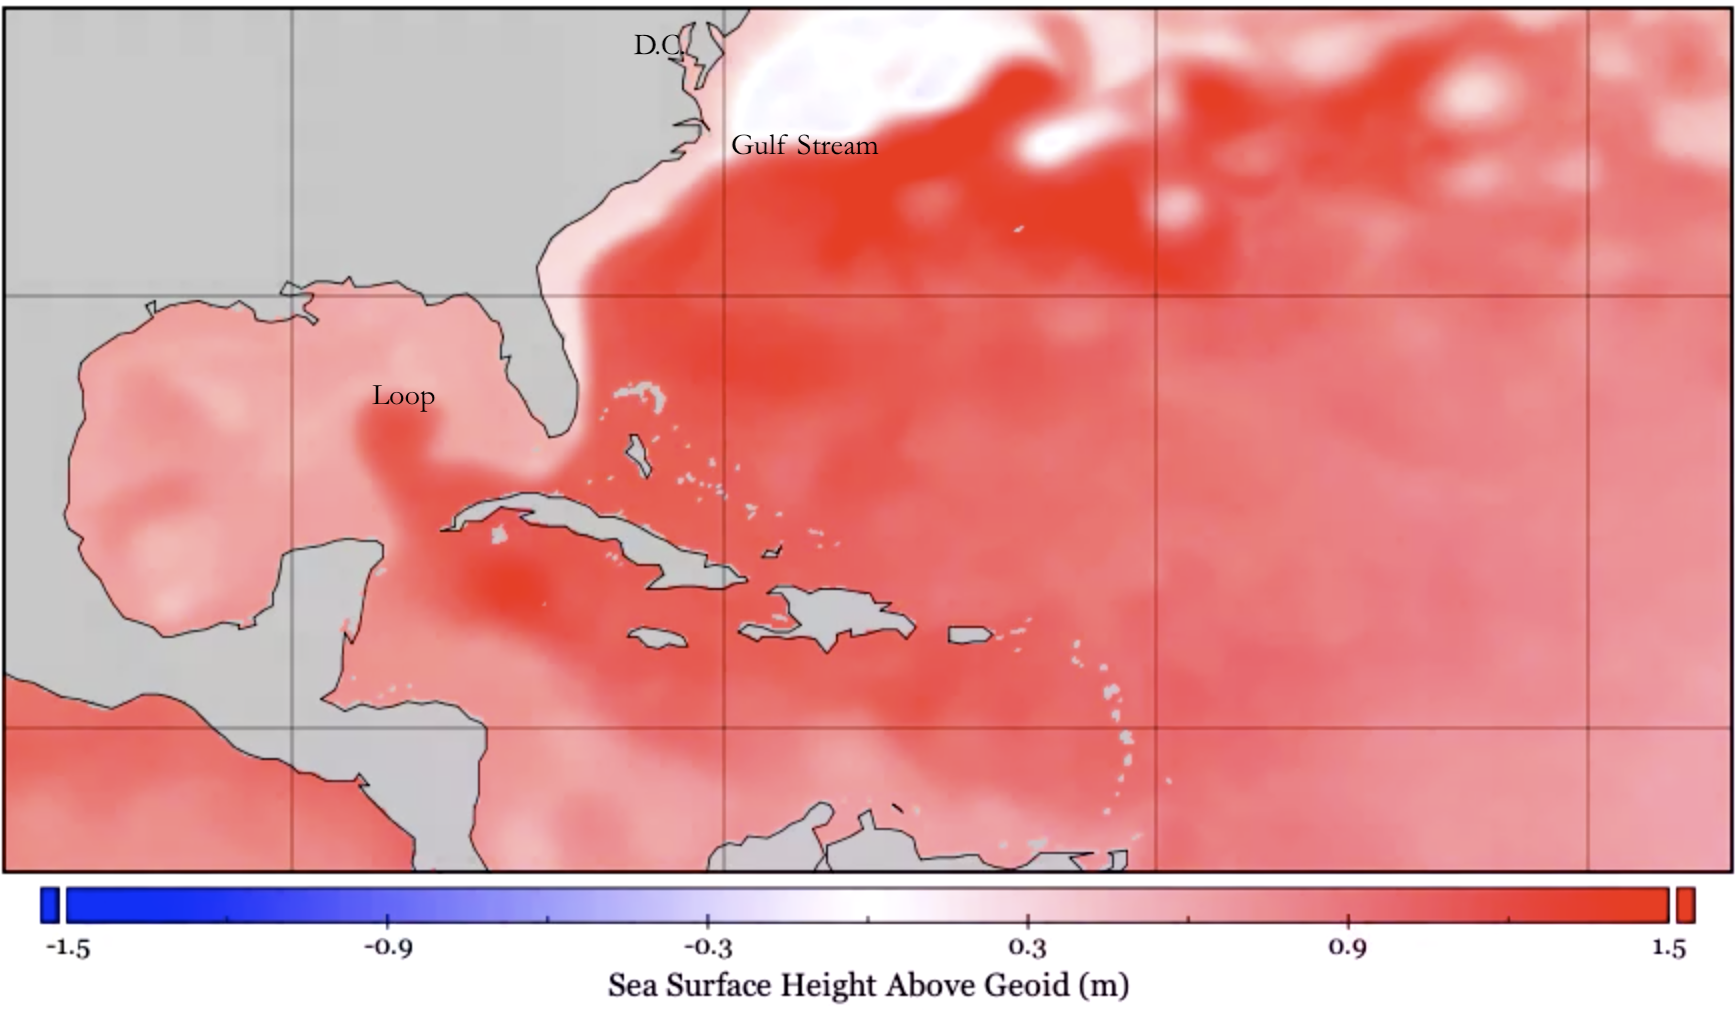
\includegraphics[width=0.93\linewidth]{images/example-images/zos-image.png}
      \end{beamercolorbox}
      \vfill
  \end{frame}

  \begin{frame}{$\eta$ Covariance and Correlation matrices are similar. }
\vspace{-20pt}
\begin{figure}[htb!]
    \centering
    \hspace{-10pt}
    \includegraphics[width=0.68\linewidth]{../surge/plots/corr_cov.pdf}
            \includegraphics[width=0.16\linewidth]{../surge/plots/corr_cov_cbar.pdf}
    \vspace{-7pt}
    \caption{A/B: Covariance matrices for 2004/5.\\
             $\quad\quad\quad\;\;$C/D: Correlation matrices for 2004/5.}
    \label{fig:}
\end{figure}
\end{frame}

\begin{frame}{ $\eta$ (SSH/zos) similar between 2004/5 }
\vspace{-20pt}
\begin{figure}[htb!]
    \centering
    \includegraphics[width=0.6\linewidth]{../surge/plots/stats_points_plot.pdf}
       \hspace{0pt} \includegraphics[width=0.285\linewidth]{../surge/plots/stats_points_plot_1.pdf}
    \vspace{-7pt}
    \caption{A comparison between the distributions of sea surface height
     above geoid (zos) for the training set (2005) and the test set (2004).}
   % \label{fig:}
\end{figure}
\end{frame}

\begin{frame}{$\eta$ No clear discontinuity between 2004/5  }
\vspace{-20pt}
\begin{figure}[htb!]
    \centering
    \includegraphics[width=0.95\linewidth]{../surge/plots/stats_points_plot_2.pdf}
    \vspace{-7pt}
    \caption{An attempt to check whether there are discontinuities
     over the special points, to explain the offsets of the means.}
    %\label{fig:}
\end{figure}
\end{frame}

\begin{frame}{Spin up may explain displacement in $\eta$ . }
\vspace{-20pt}
\begin{figure}[htb!]
    \centering
    \includegraphics[width=0.95\linewidth]{../surge/plots/stats_points_plot_5.pdf}
    \vspace{-7pt}
    \caption{Early months in 2004 do not seem
             to follow the yearly pattern followed elsewhere.}
    %\label{fig:A}
\end{figure}
\end{frame}


\begin{frame}{Gaussian Processes Refresher}
\vspace{-20pt}
\begin{itemize}
\item Equations 2.13-2.14 in GPML~\cite{williams2006gaussian}.
\begin{align}
m(\mathbf{x})&=&\mathbb{E}[f(\mathbf{x})] % \tag{Mean}
\\
k\left(\mathbf{x}, \mathbf{x}^{\prime}\right)&=&\mathbb{E}
\left[(f(\mathbf{x})-m(\mathbf{x}))\left(f\left(\mathbf{x}^{\prime}\right)
-m\left(\mathbf{x}^{\prime}\right)\right)\right]
%\tag{Covariance}
\\
f(\mathbf{x})& \sim& \mathcal{G} \mathcal{P}\left(m(\mathbf{x}),
 k\left(\mathbf{x}, \mathbf{x}^{\prime}\right)\right)%\tag{GP}
\end{align}
\item Can assume $m(\mathbf{x})=0$ without terrible consequences.
 \item Thought should be put into the form of $k\left(\mathbf{x},
  \mathbf{x}^{\prime}\right)$~\cite{duvenaud2014automatic}.
\end{itemize}
\end{frame}

\begin{frame}{Warped Gaussian Processes}
\vspace{-20pt}
\begin{itemize}
\item GPs assume that there is a Gaussian error around each point,
      but this is often not the case in real variables.
      However, it is often possible to transform to
      a space where this is the case, Krige there,
      and then transform
      back~\cite{snelson2004warped}.\footnote{\url{http://mlg.eng.cam.ac.uk/zoubin/papers/gpwarp.pdf}}
      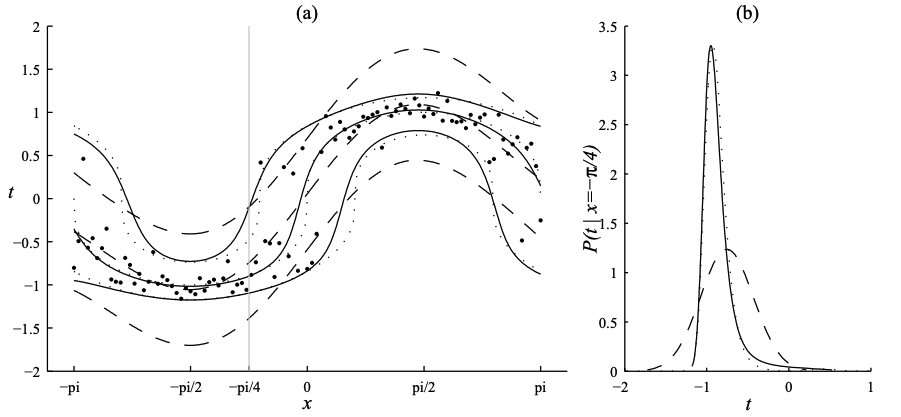
\includegraphics[width=0.7\linewidth]{images/example-images/warped-example.png}\\
      \textit{Figure 1 from~\cite{snelson2004warped}}
\item Lewis Fry Richardson (1948) showed that the estimates
      of deaths during a war had
      symmetric error bars in logarithmic space~\cite{richardson1948variation}.
      \cite{snelson2004warped}~mentions this as a common trick.
 \end{itemize}

\end{frame}


\begin{frame}{There is a strong yearly periodicity in $\eta$. }
\vspace{-20pt}
\begin{figure}[htb!]
    \centering
    \includegraphics[width=0.95\linewidth]{../surge/plots/ahh/ahhhhh4.pdf}
    \vspace{-7pt}
    \caption{There is a strong yearly periodicity in $\eta$ (and its variance?).
     Kriged with a Sobol quasirandom subsample~\cite{sobol1967distribution} of 6000 points.}
    %\label{fig:A}
\end{figure}
\end{frame}


\begin{frame}{There is  supported by taking the Fourier Transform }
\vspace{-40pt}
\begin{figure}[htb!]
    \centering
    \begin{equation}
F(f)=\int_{-\infty}^{\infty} y(x) e^{-i 2\pi f x} d x
\end{equation}
\begin{equation}
\sum_{n=0}^{N-1} a_{n} e^{-2 \pi i  k n/ N}=\sum_{n=0}^{N / 2-1} a_{2 n}
e^{-2 \pi i k (2 n)/ N} +\sum_{n=0}^{N / 2-1} a_{2n+1} e^{-2 \pi i k (2 n+1)/ N}
\end{equation}
    \includegraphics[width=0.85\linewidth]{../surge/plots/fourier_transform_grid.pdf}
    \vspace{-7pt}
    \caption{Fourier Transform~\cite{cooley1965algorithm} of $\Delta\eta$ by coastal point.}
    % \label{fig:A}
\end{figure}
\end{frame}


\begin{frame}[fragile]{Low / High Pass Filter of New Orleans }
\vspace{-10pt}
    %\centering
\begin{block}{Fast Fourier Transform (1) and Its Inverse (2)}
\vspace{-10pt}
\begin{lstlisting}[firstnumber=1, language=python, label=glabels, xleftmargin=0pt]
y(j) = (x * exp(-2*pi*sqrt(-1)*j*np.arange(n)/n)).sum()
y(j) = (x * exp(2*pi*sqrt(-1)*j*np.arange(n)/n)).mean()
\end{lstlisting}
\end{block}
\vspace{-30pt}
\begin{figure}[htb!]
\begin{equation}
\Delta\eta_{\;\mathrm{lp}}(t) = \int_{\mathbb{R}}W\left(\frac{|f|}
{|f|_{\mathrm{thresh}}}\right)\int_{\mathbb{R}}e^{2\pi i
(t-t^{\prime})f }\Delta \eta(t^{\prime})dt^{\prime}df
\end{equation}
\begin{equation}
\Delta\eta_{\;\mathrm{hp}}(t) = \int_{\mathbb{R}}\left(1-W\left(\frac{|f|}
{|f|_{\mathrm{thresh}}}\right)\right)\int_{\mathbb{R}}e^{2\pi i
(t-t^{\prime})f }\Delta \eta(t^{\prime})dt^{\prime}df
\end{equation}
    \centering
    \includegraphics[width=0.95\linewidth]{../surge/plots/norlean-low-pass.pdf}
    \vspace{-15pt}
    \caption{Fourier Transform~\cite{cooley1965algorithm} of $\Delta\eta$ for New Orleans.}
    \label{fig:A}
\end{figure}
\end{frame}

\begin{frame}[fragile]{Low / High Pass Filter of Miami }
\vspace{-10pt}
    %\centering
\begin{block}{Fast Fourier Transform (1) and Its Inverse (2)}
\vspace{-10pt}
\begin{lstlisting}[firstnumber=1, language=python, label=glabels, xleftmargin=0pt]
y(j) = (x * exp(-2*pi*sqrt(-1)*j*np.arange(n)/n)).sum()
y(j) = (x * exp(2*pi*sqrt(-1)*j*np.arange(n)/n)).mean()
\end{lstlisting}
\end{block}
\vspace{-30pt}
\begin{figure}[htb!]
\begin{equation}
\Delta\eta_{\;\mathrm{lp}}(t) = \int_{\mathbb{R}}W\left(\frac{|f|}
{|f|_{\mathrm{thresh}}}\right)\int_{\mathbb{R}}e^{2\pi i (t-t^{\prime})f }
\Delta \eta(t^{\prime})dt^{\prime}df
\end{equation}
\begin{equation}
\Delta\eta_{\;\mathrm{hp}}(t) = \int_{\mathbb{R}}\left(1-W\left(\frac{|f|}
{|f|_{\mathrm{thresh}}}\right)\right)\int_{\mathbb{R}}e^{2\pi i (t-t^{\prime})f}
   \Delta \eta(t^{\prime})dt^{\prime}df
\end{equation}
    \centering
    \includegraphics[width=0.95\linewidth]{../surge/plots/mm-low-pass.pdf}
    \vspace{-15pt}
    \caption{Fourier Transform~\cite{cooley1965algorithm} of $\Delta\eta$ for Miami.}
    \label{fig:A}
\end{figure}
\end{frame}

\begin{frame}[fragile]{Low / High Pass Filter of New York }
\vspace{-30pt}
    %\centering
\begin{block}{Fast Fourier Transform (1) and Its Inverse (2)}
\begin{lstlisting}[firstnumber=1, language=python, label=glabels, xleftmargin=0pt]
y(j) = (x * exp(-2*pi*sqrt(-1)*j*np.arange(n)/n)).sum()
y(j) = (x * exp(2*pi*sqrt(-1)*j*np.arange(n)/n)).mean()
\end{lstlisting}
\end{block}
\vspace{-20pt}
\begin{figure}[htb!]
    \centering
    \includegraphics[width=0.95\linewidth]{../surge/plots/ny-low-pass.pdf}
    \vspace{-7pt}
    \caption{Fourier Transform~\cite{cooley1965algorithm} of $\Delta\eta$ for New York.}
    \label{fig:A}
\end{figure}
\end{frame}


\begin{frame}{Low / High Pass Filter for all Points}
\vspace{-30pt}
    %\centering
\hspace{-30pt}
 \begin{minipage}{1.15\textwidth}
\begin{figure}[htb!]
    \centering
   \hspace{-40pt} \includegraphics[width=0.48\linewidth]{../surge/plots/low_pass_grid.pdf}
        \includegraphics[width=0.48\linewidth]{../surge/plots/high_pass_grid.pdf}
    \vspace{-7pt}
    \caption{Fourier Transform~\cite{cooley1965algorithm} of $\Delta\eta$}
    \label{fig:A}
\end{figure}
\end{minipage}
\end{frame}


\begin{frame}{$|f|_{thresh}=2$ yr$^{-1}$ Maximises Linear Predictability }
\centering

Linear Predictability (LP) defined in next section

    \hspace{-30pt}\begin{minipage}{0.57\textwidth}
    \begin{figure}
            \includegraphics[width=1\linewidth]{../surge/plots/reg_fft/up_to_100_full_coast.pdf}
                \caption{LP for each point.}
    \end{figure}

    \end{minipage}\hspace{5pt}
      \begin{minipage}{0.45\textwidth}
\begin{figure}[htb!]
    \centering
    \includegraphics[width=1\linewidth]{../surge/plots/reg_fft/up_to_100_coastal_average.pdf}
    \caption{Averaged over points.}
    \label{fig:}
\end{figure}
    \end{minipage}
\end{frame}
